\chapter{Actual Evaluation Instruments (Survey / Questionnaire Forms)}
\label{app:actual_evaluation_instruments}
\addcontentsline{toc}{chapter}{Actual Evaluation Instruments (Survey / Questionnaire Forms)}

\section*{Common Sections: All Respondent Groups}

\subsection*{Introduction, Informed Consent, and Respondent Profile}

\begin{center}
\begin{minipage}{\textwidth}
    \centering
    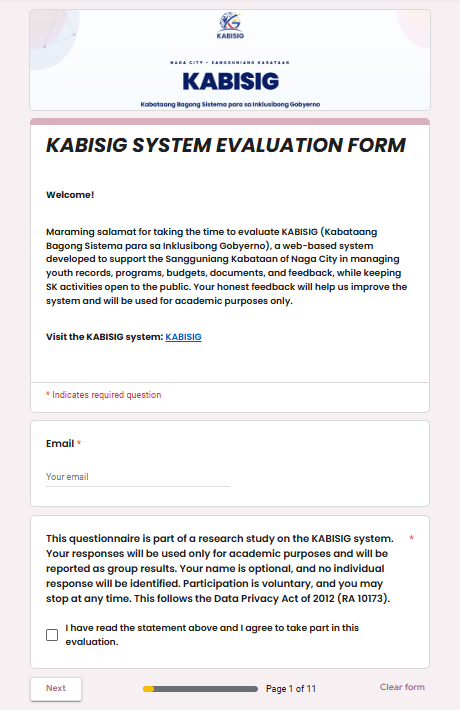
\includegraphics[height=0.38\textheight]{figures/p1}
    \par\smallskip
    {\small \textbf{Figure F.1:} Welcome screen, required email field, and informed consent statement.}
\end{minipage}
\end{center}

\begin{center}
\begin{minipage}{\textwidth}
    \centering
    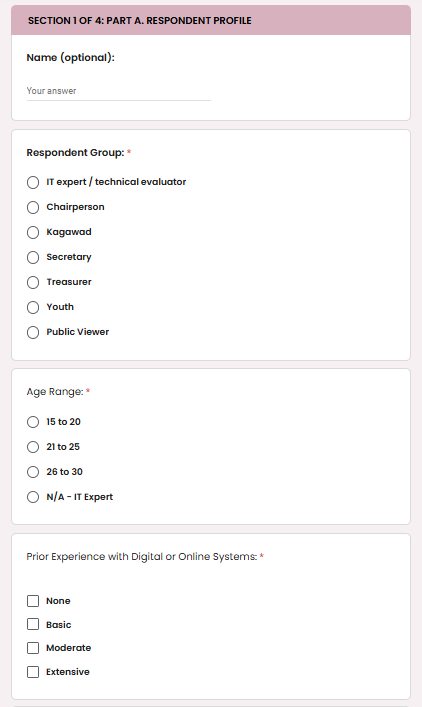
\includegraphics[height=0.38\textheight]{figures/p2}
    \par\smallskip
    {\small \textbf{Figure F.2:} Part A respondent profile fields, respondent group, age range, and prior digital experience.}
\end{minipage}
\end{center}

\begin{center}
\begin{minipage}{\textwidth}
    \centering
    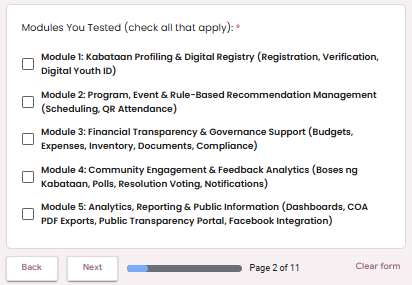
\includegraphics[height=0.36\textheight]{figures/p3}
    \par\smallskip
    {\small \textbf{Figure F.3:} Tested modules checklist across Modules 1 through 5.}
\end{minipage}
\end{center}

\clearpage
\section*{Part 1: IT Experts \& Technical Evaluators Section (ISO/IEC 25010:2023)}
\begin{center}
\begin{minipage}{\textwidth}
    \centering
    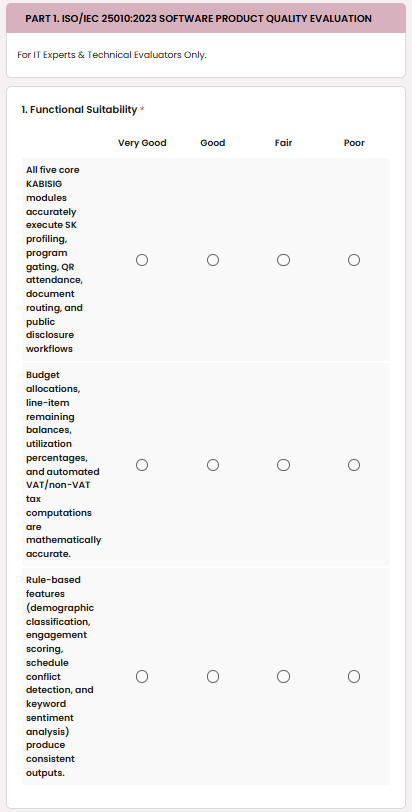
\includegraphics[height=0.38\textheight]{figures/itp1}
    \par\smallskip
    {\small \textbf{Figure F.4:} ISO/IEC 25010:2023 Functional Suitability evaluation items assessing core module workflows, financial computations, and rule-based outputs.}
\end{minipage}
\end{center}

\begin{center}
\begin{minipage}{\textwidth}
    \centering
    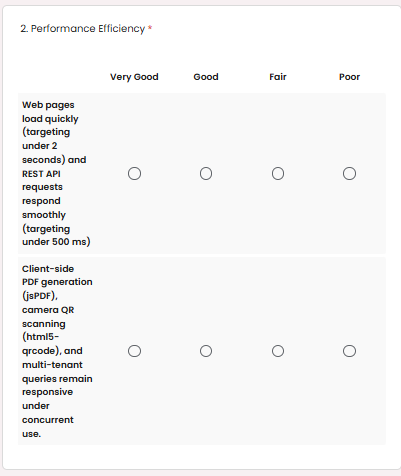
\includegraphics[height=0.38\textheight]{figures/itp2}
    \par\smallskip
    {\small \textbf{Figure F.5:} ISO/IEC 25010:2023 Performance Efficiency evaluation items measuring page load speed, API response times, and concurrent client-side processing.}
\end{minipage}
\end{center}

\begin{center}
\begin{minipage}{\textwidth}
    \centering
    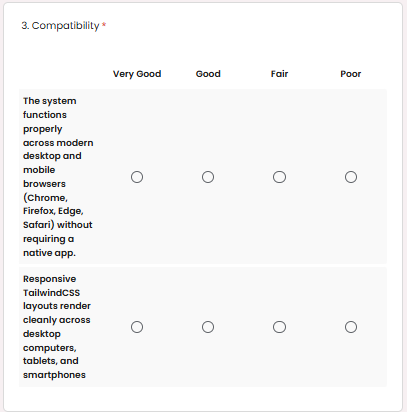
\includegraphics[height=0.38\textheight]{figures/itp3}
    \par\smallskip
    {\small \textbf{Figure F.6:} ISO/IEC 25010:2023 Compatibility evaluation items verifying cross-browser operation and responsive layouts across devices.}
\end{minipage}
\end{center}

\begin{center}
\begin{minipage}{\textwidth}
    \centering
    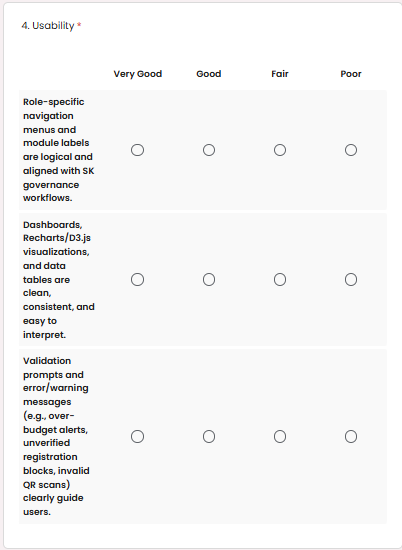
\includegraphics[height=0.38\textheight]{figures/itp4}
    \par\smallskip
    {\small \textbf{Figure F.7:} ISO/IEC 25010:2023 Usability evaluation items covering role-based navigation, data visualizations, and validation prompts.}
\end{minipage}
\end{center}

\begin{center}
\begin{minipage}{\textwidth}
    \centering
    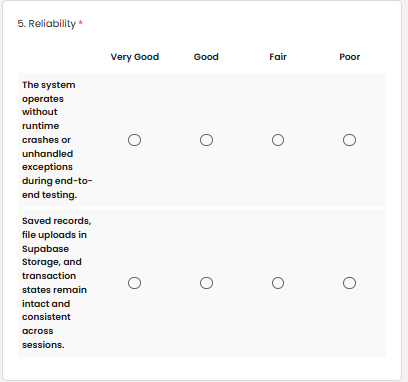
\includegraphics[height=0.38\textheight]{figures/itp5}
    \par\smallskip
    {\small \textbf{Figure F.8:} ISO/IEC 25010:2023 Reliability evaluation items assessing runtime stability and persistent data integrity across sessions.}
\end{minipage}
\end{center}

\begin{center}
\begin{minipage}{\textwidth}
    \centering
    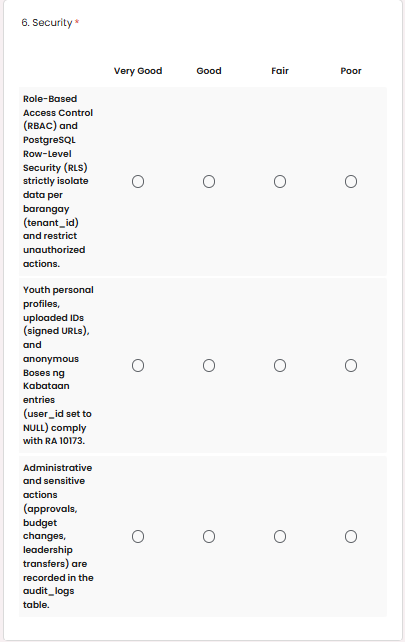
\includegraphics[height=0.38\textheight]{figures/itp6}
    \par\smallskip
    {\small \textbf{Figure F.9:} ISO/IEC 25010:2023 Security evaluation items verifying multi-tenant row-level isolation, RA 10173 data privacy compliance, and audit logging.}
\end{minipage}
\end{center}

\begin{center}
\begin{minipage}{\textwidth}
    \centering
    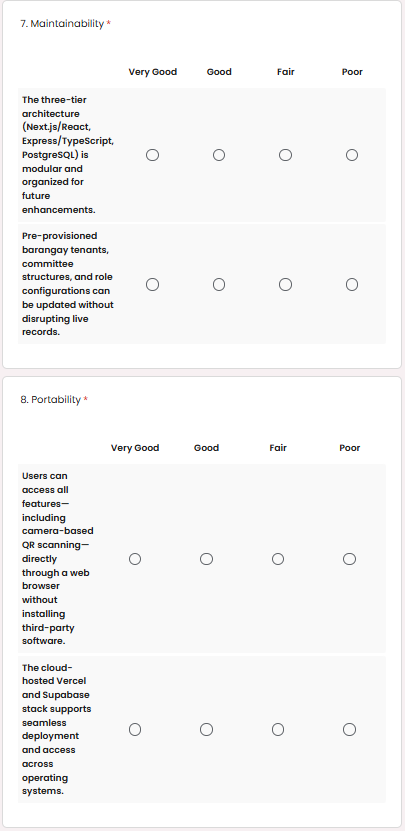
\includegraphics[height=0.38\textheight]{figures/itp7-8}
    \par\smallskip
    {\small \textbf{Figure F.10:} ISO/IEC 25010:2023 Maintainability and Portability evaluation items assessing modular code structure, deployment readiness, and environment adaptability.}
\end{minipage}
\end{center}

\begin{center}
\begin{minipage}{\textwidth}
    \centering
    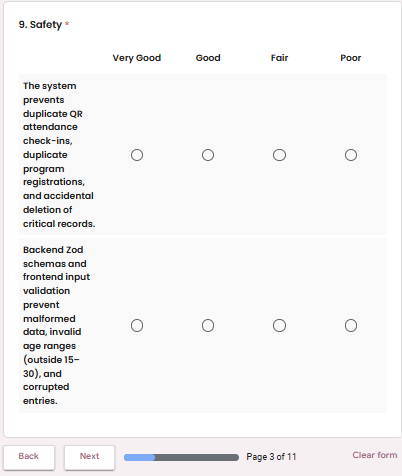
\includegraphics[height=0.38\textheight]{figures/itp9}
    \par\smallskip
    {\small \textbf{Figure F.11:} Overall technical assessment and final evaluation items for IT experts and technical evaluators.}
\end{minipage}
\end{center}

\section*{PART 2. TECHNOLOGY ACCEPTANCE MODEL (TAM) EVALUATION BY ROLE}
\clearpage
\section*{SK Chairperson Section}

\begin{center}
\begin{minipage}{\textwidth}
    \centering
    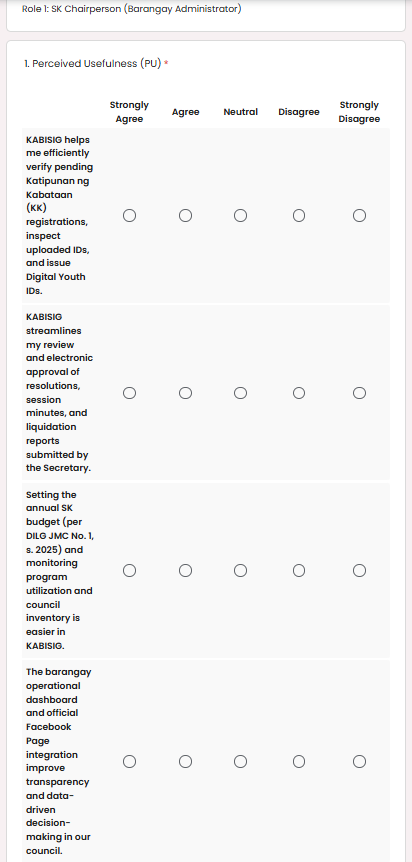
\includegraphics[height=0.38\textheight]{figures/cp1}
    \par\smallskip
    {\small \textbf{Figure F.12:} Perceived Usefulness (PU) items for SK Chairpersons covering KK registration verification, document and liquidation approvals, DILG budget monitoring, and council transparency.}
\end{minipage}
\end{center}

\begin{center}
\begin{minipage}{\textwidth}
    \centering
    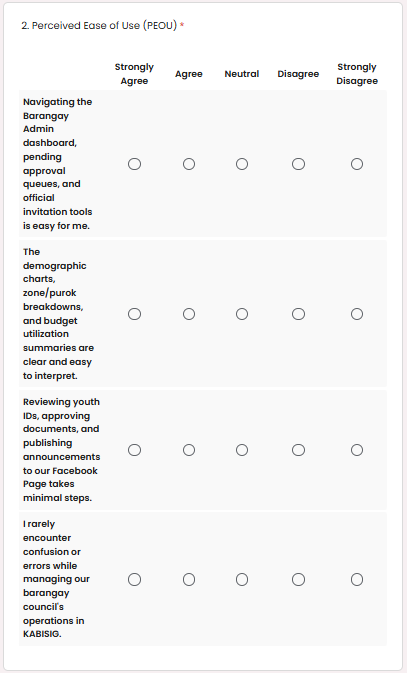
\includegraphics[height=0.38\textheight]{figures/cp2}
    \par\smallskip
    {\small \textbf{Figure F.13:} Perceived Ease of Use (PEOU) items for SK Chairpersons assessing navigation of the Barangay Admin dashboard, analytics summaries, approval workflows, and error-free operation.}
\end{minipage}
\end{center}

\begin{center}
\begin{minipage}{\textwidth}
    \centering
    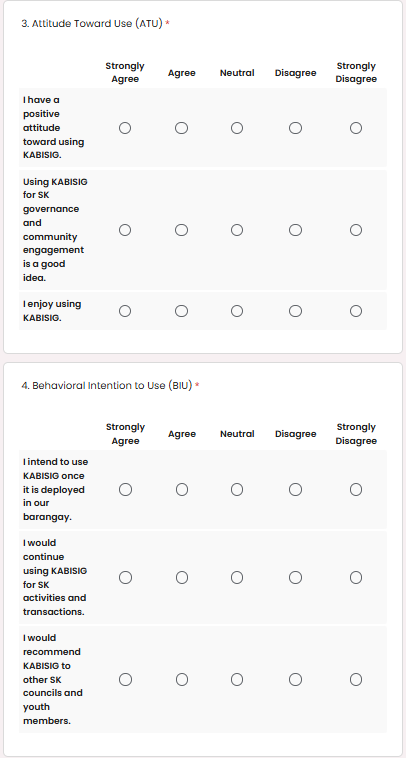
\includegraphics[height=0.38\textheight]{figures/cp3-4}
    \par\smallskip
    {\small \textbf{Figure F.14:} Attitude Toward Use (ATU) and Behavioral Intention to Use (BIU) items measuring SK Chairpersons' positive outlook, enjoyment, post-deployment adoption intent, and willingness to recommend KABISIG.}
\end{minipage}
\end{center}

\clearpage
\section*{SK Kagawad Section}

\begin{center}
\begin{minipage}{\textwidth}
    \centering
    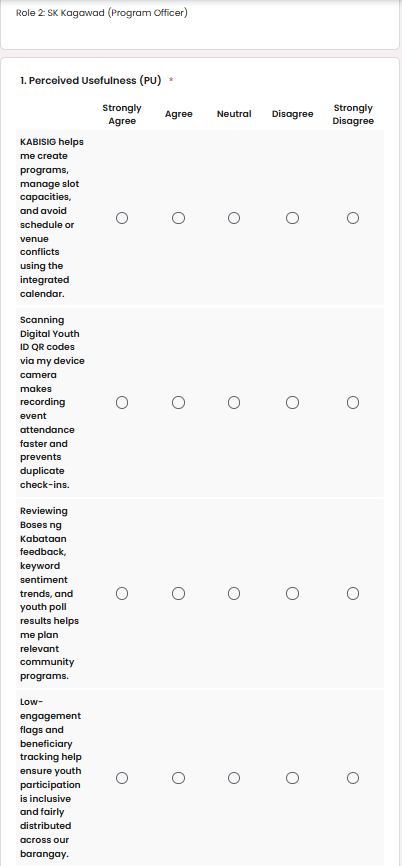
\includegraphics[height=0.38\textheight]{figures/kp1}
    \par\smallskip
    {\small \textbf{Figure F.15:} Perceived Usefulness (PU) items for SK Kagawad covering program scheduling and conflict avoidance, QR attendance scanning, feedback and sentiment review, and inclusive beneficiary tracking.}
\end{minipage}
\end{center}

\begin{center}
\begin{minipage}{\textwidth}
    \centering
    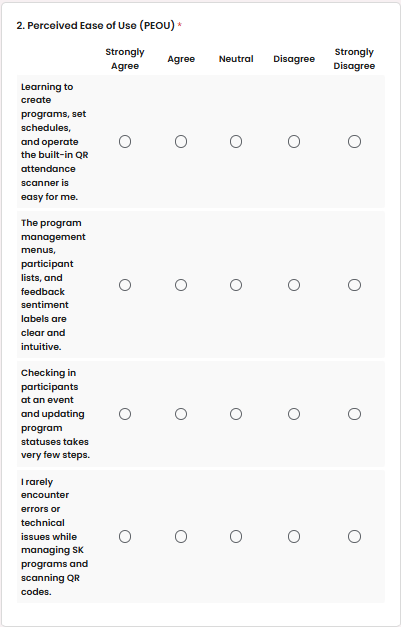
\includegraphics[height=0.38\textheight]{figures/kp2}
    \par\smallskip
    {\small \textbf{Figure F.16:} Perceived Ease of Use (PEOU) items for SK Kagawad assessing ease of creating programs, intuitive menus and labels, streamlined check-ins, and minimal errors during program and QR operations.}
\end{minipage}
\end{center}

\begin{center}
\begin{minipage}{\textwidth}
    \centering
    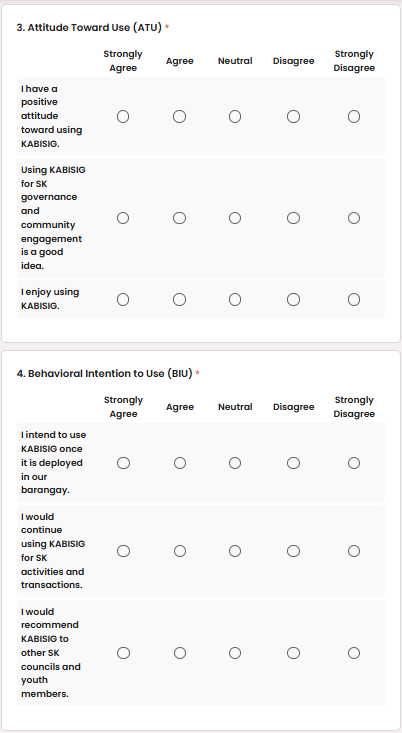
\includegraphics[height=0.38\textheight]{figures/kp3-4}
    \par\smallskip
    {\small \textbf{Figure F.17:} Attitude Toward Use (ATU) and Behavioral Intention to Use (BIU) items measuring SK Kagawad's positive attitude, enjoyment, post-deployment adoption intent, and recommendation willingness.}
\end{minipage}
\end{center}

\clearpage
\section*{SK Secretary Section}

\begin{center}
\begin{minipage}{\textwidth}
    \centering
    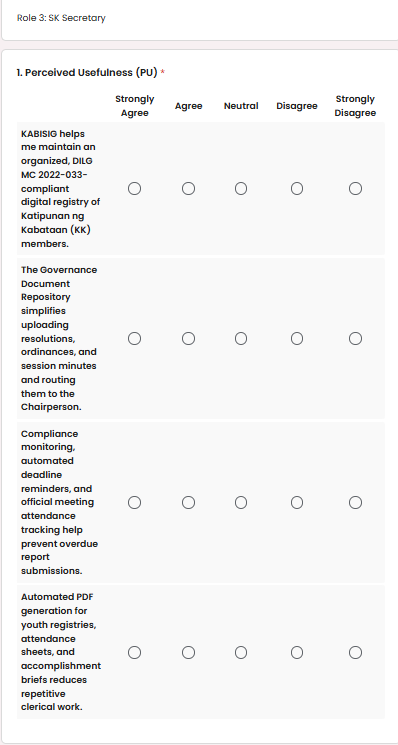
\includegraphics[height=0.38\textheight]{figures/sp1}
    \par\smallskip
    {\small \textbf{Figure F.18:} Perceived Usefulness (PU) items for SK Secretaries covering KK registry management, governance document routing, compliance and deadline tracking, and automated PDF report generation.}
\end{minipage}
\end{center}

\begin{center}
\begin{minipage}{\textwidth}
    \centering
    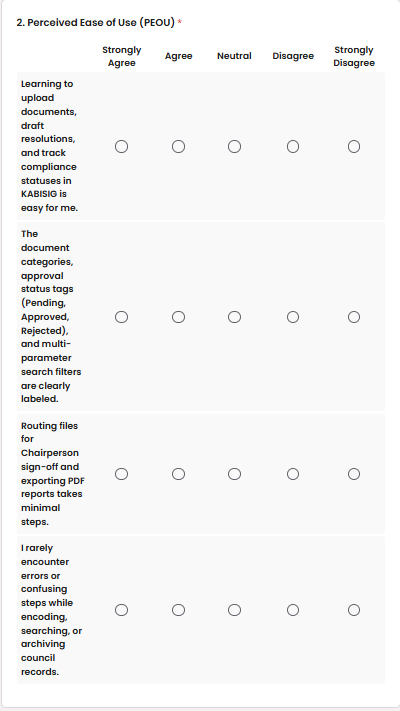
\includegraphics[height=0.38\textheight]{figures/sp2}
    \par\smallskip
    {\small \textbf{Figure F.19:} Perceived Ease of Use (PEOU) items for SK Secretaries assessing ease of uploading and filtering documents, clear status labels, streamlined routing and PDF exports, and minimal record-encoding errors.}
\end{minipage}
\end{center}

\begin{center}
\begin{minipage}{\textwidth}
    \centering
    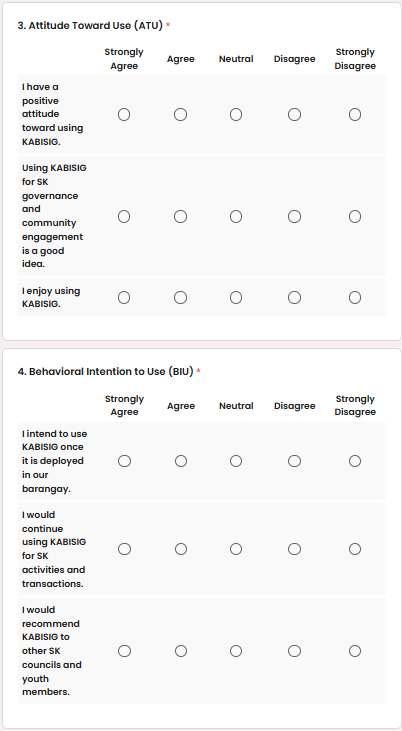
\includegraphics[height=0.38\textheight]{figures/sp3}
    \par\smallskip
    {\small \textbf{Figure F.20:} Attitude Toward Use (ATU) and Behavioral Intention to Use (BIU) items measuring SK Secretaries' positive attitude, enjoyment, post-deployment adoption intent, and recommendation willingness.}
\end{minipage}
\end{center}

\clearpage
\section*{SK Treasurer Section}

\begin{center}
\begin{minipage}{\textwidth}
    \centering
    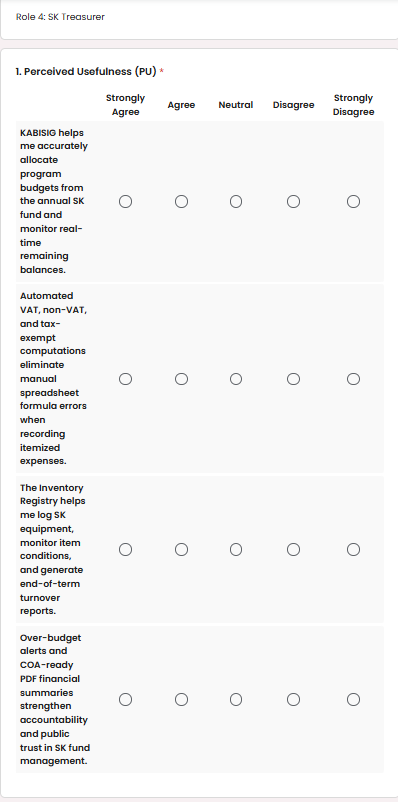
\includegraphics[height=0.38\textheight]{figures/tp1}
    \par\smallskip
    {\small \textbf{Figure F.21:} Perceived Usefulness (PU) items for SK Treasurers covering annual SK fund allocation and real-time balance tracking, automated VAT and tax calculations, equipment inventory and turnover logs, and over-budget alerts with COA-ready PDF summaries.}
\end{minipage}
\end{center}

\begin{center}
\begin{minipage}{\textwidth}
    \centering
    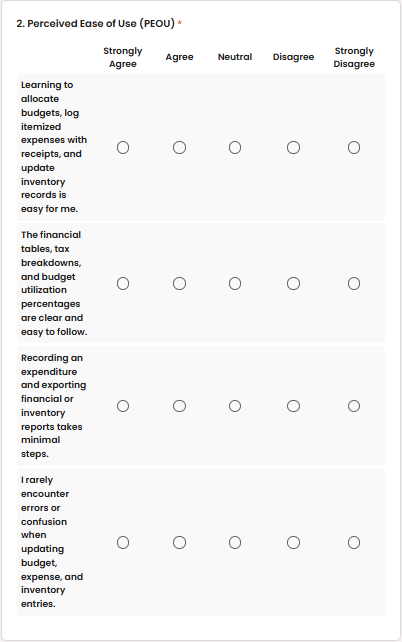
\includegraphics[height=0.38\textheight]{figures/tp2}
    \par\smallskip
    {\small \textbf{Figure F.22:} Perceived Ease of Use (PEOU) items for SK Treasurers assessing ease of budget allocation, expense logging with receipts, and inventory updates, clear financial tables and utilization metrics, minimal export steps, and low entry errors.}
\end{minipage}
\end{center}

\begin{center}
\begin{minipage}{\textwidth}
    \centering
    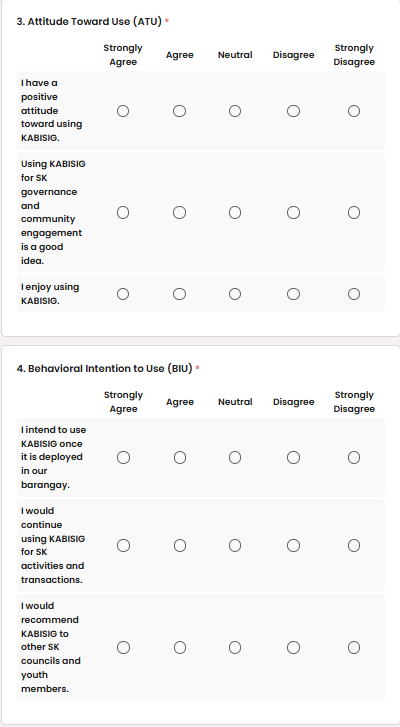
\includegraphics[height=0.38\textheight]{figures/tp3}
    \par\smallskip
    {\small \textbf{Figure F.23:} Attitude Toward Use (ATU) and Behavioral Intention to Use (BIU) items measuring SK Treasurers' positive attitude, enjoyment, post-deployment adoption intent, and recommendation willingness.}
\end{minipage}
\end{center}

\clearpage
\section*{Youth Section}

\begin{center}
\begin{minipage}{\textwidth}
    \centering
    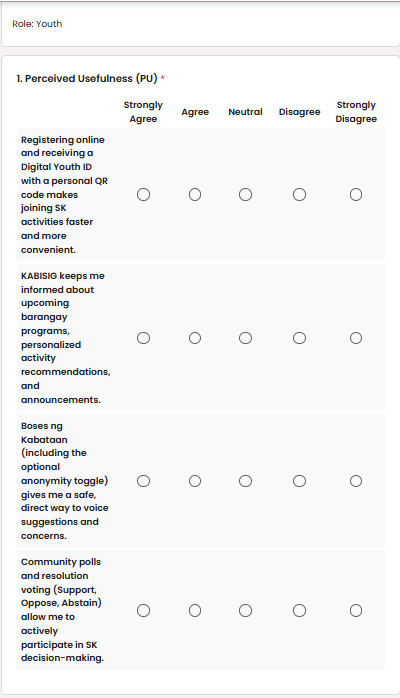
\includegraphics[height=0.38\textheight]{figures/yp1}
    \par\smallskip
    {\small \textbf{Figure F.24:} Perceived Usefulness (PU) items for Youth respondents covering online registration and Digital Youth ID QR access, upcoming program updates and recommendations, anonymous \textit{Boses ng Kabataan} feedback, and community polls and resolution voting.}
\end{minipage}
\end{center}

\begin{center}
\begin{minipage}{\textwidth}
    \centering
    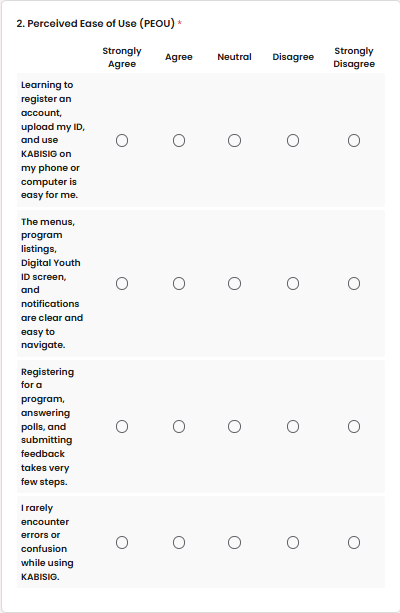
\includegraphics[height=0.38\textheight]{figures/yp2}
    \par\smallskip
    {\small \textbf{Figure F.25:} Perceived Ease of Use (PEOU) items for Youth respondents assessing ease of account registration and ID upload, clear Digital Youth ID and program navigation, minimal steps for joining activities and polls, and error-free operation.}
\end{minipage}
\end{center}

\begin{center}
\begin{minipage}{\textwidth}
    \centering
    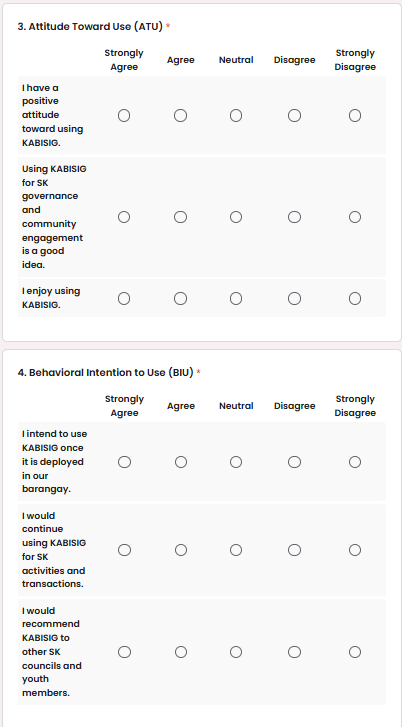
\includegraphics[height=0.38\textheight]{figures/yp3}
    \par\smallskip
    {\small \textbf{Figure F.26:} Attitude Toward Use (ATU) and Behavioral Intention to Use (BIU) items measuring Youth respondents' positive attitude, enjoyment, post-deployment adoption intent, and willingness to recommend KABISIG.}
\end{minipage}
\end{center}

\clearpage
\section*{Public Viewer Section}

\begin{center}
\begin{minipage}{\textwidth}
    \centering
    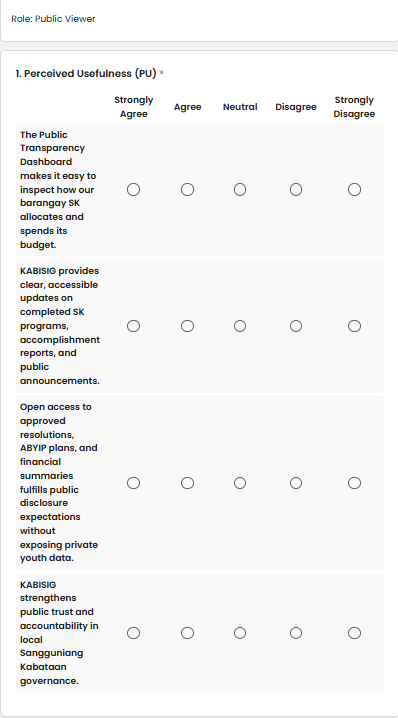
\includegraphics[height=0.38\textheight]{figures/pp1}
    \par\smallskip
    {\small \textbf{Figure F.27:} Perceived Usefulness (PU) items for Public Viewers covering inspection of barangay SK budget allocations and spending, accessible updates on completed programs and announcements, public disclosure of approved resolutions and ABYIP plans without exposing private youth data, and strengthened public trust in SK governance.}
\end{minipage}
\end{center}

\begin{center}
\begin{minipage}{\textwidth}
    \centering
    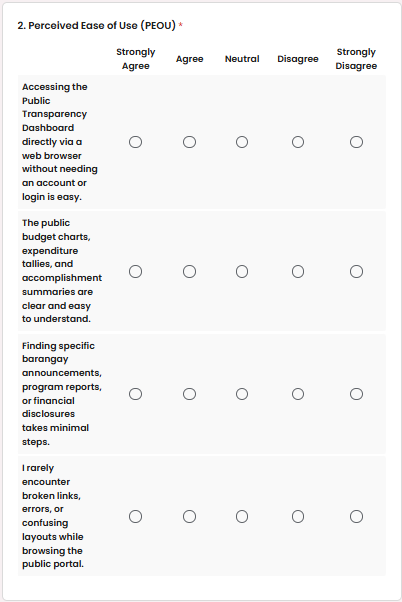
\includegraphics[height=0.38\textheight]{figures/pp2}
    \par\smallskip
    {\small \textbf{Figure F.28:} Perceived Ease of Use (PEOU) items for Public Viewers assessing login-free web browser access to the Public Transparency Dashboard, clear budget charts and accomplishment summaries, minimal steps to locate reports and disclosures, and error-free public portal navigation.}
\end{minipage}
\end{center}

\begin{center}
\begin{minipage}{\textwidth}
    \centering
    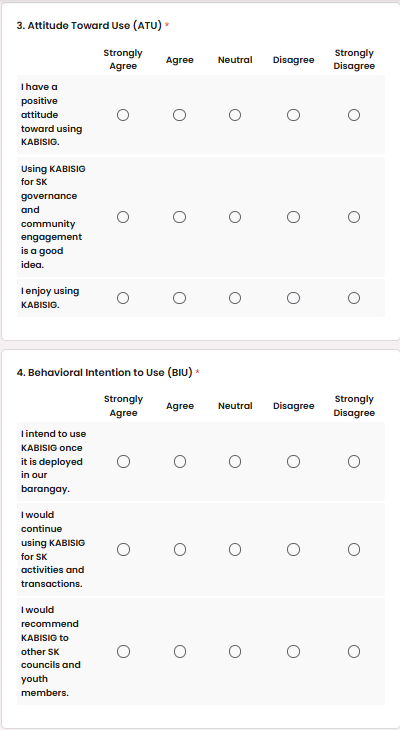
\includegraphics[height=0.38\textheight]{figures/pp3-4}
    \par\smallskip
    {\small \textbf{Figure F.29:} Attitude Toward Use (ATU) and Behavioral Intention to Use (BIU) items measuring Public Viewers' positive attitude, enjoyment, post-deployment adoption intent, and willingness to recommend KABISIG.}
\end{minipage}
\end{center}


\clearpage
\section*{Part 3. QUALITATIVE FEEDBACK (All Respondents)}

\begin{center}
\begin{minipage}{\textwidth}
    \centering
    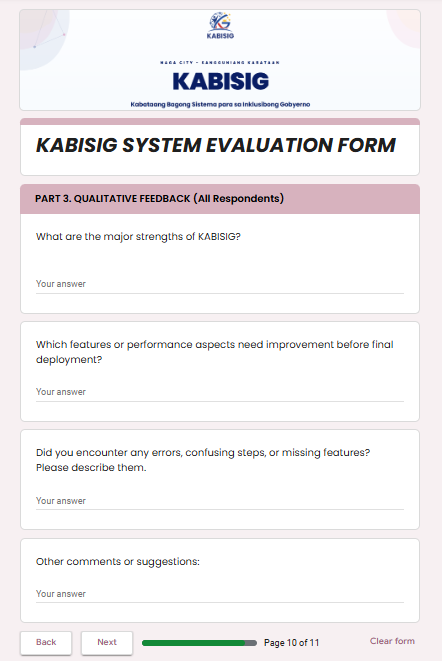
\includegraphics[height=0.45\textheight]{figures/itlast}
    \par\smallskip
    {\small \textbf{Figure F.30:} Open-ended qualitative feedback questions capturing system strengths, areas for improvement, encountered issues, and suggestions.}
\end{minipage}
\end{center}